\section{Analyse der Transceiver-Platinen}
Zur Verfügung steht eine Transceiver-Platine. Ein Transceiver ist eine Platine, die sowohl als Sender (Transmitter), als auch als Empfänger (Receiver) fungieren kann. Dafür ist diese Platine entsprechend bestückt, sodass die Funktion der Platine verändert werden kann. 
Hierfür stehen zwei Jumper zur Verfügung, die auf der Transceiver-Platine platziert sind. Diese können gesteckt oder abgezogen werden.
\subsection{Funktion der Jumper}
Die Jumper sind in Abbildung \ref{fig:Tranceiver-Platine} zu sehen.
\begin{figure}[H]
    \centering
    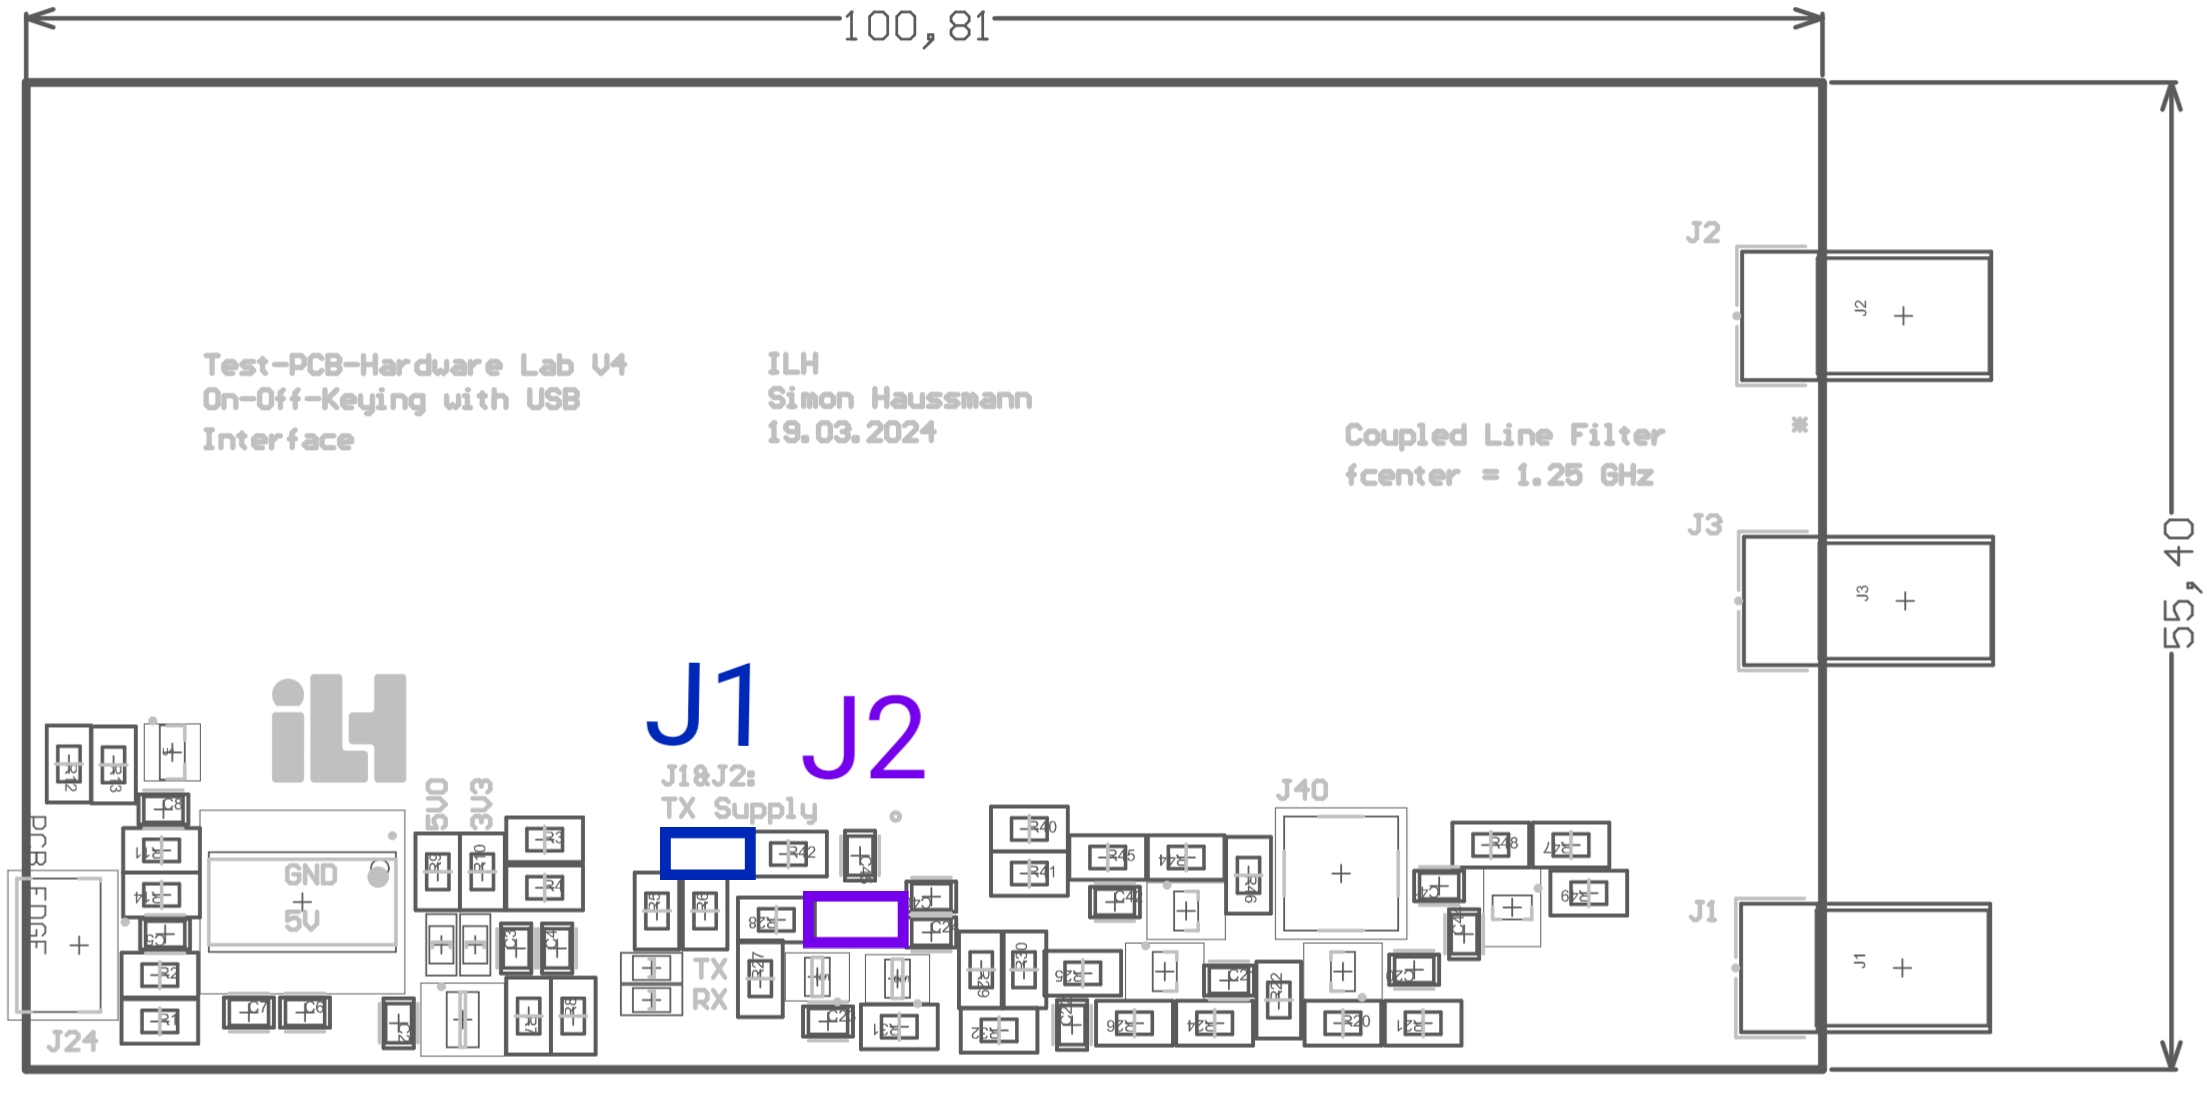
\includegraphics[width=0.8\textwidth]{Pictures/Jumper.jpg}
    \caption{Transceiver-Platine mit Jumpern J1 und J2. Quelle: vgl. Literaturverzeichnis \cite{SchaltplanPCBV4}: Schaltpläne der Platine V4}
    \label{fig:Tranceiver-Platine}
\end{figure}
\begin{figure}[H]
    \centering
    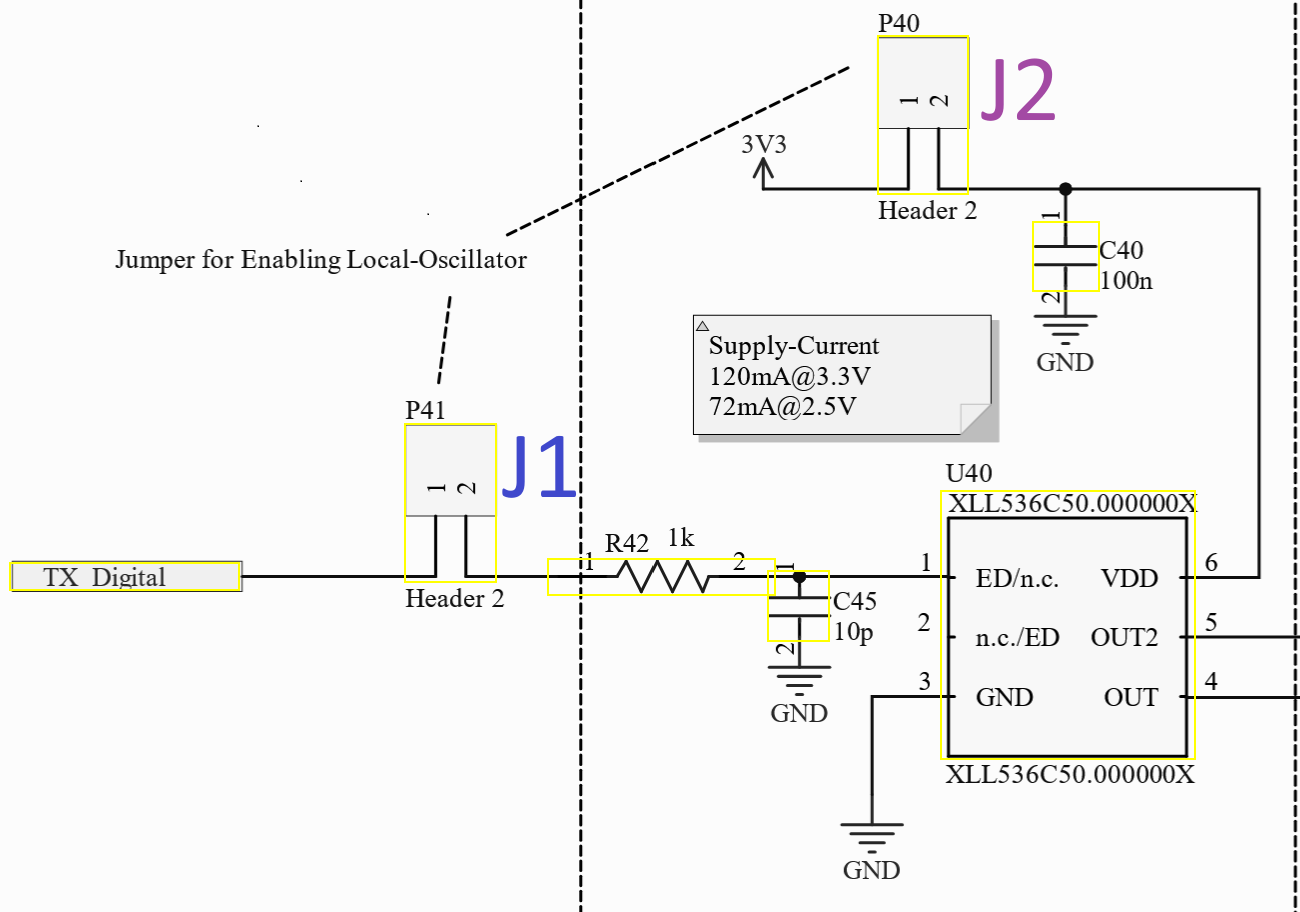
\includegraphics[width=0.8\textwidth]{Pictures/JumperSchaltung.png}
    \caption{Jumperkonfiguration}
    \label{fig:Jumper}
\end{figure}
\subsection{J1}
Der Jumper J1 ist, wie im Schaltplan zu sehen, der Schalter, der den Oszillator aktiviert und deaktiviert.
\subsection{J2}
Der Jumper J2 ist, wie im Schaltplan zu sehen, der Schalter für die Versorgungsspannung des Oszillators.

\subsection{Modi der Platine}
(\textcolor{red}{X} steht hierbei dafür, dass der Jumper entfernt ist, 
\textcolor{green}{\checkmark} dass der Jumper gesetzt ist):\\ 

\begin{table}[h!]
    \centering
    \begin{tabular}{|c|c|c|}
        \hline
          J1 & J2 & Funktion \\
        \hline
         \textcolor{red}{X} & \textcolor{green}{\checkmark} & Sender ohne Datensignal\\
          \textcolor{green}{\checkmark}& \textcolor{green}{\checkmark} & Sender mit Datensignal(PC)\\
        \textcolor{red}{X} & \textcolor{red}{X} & Empfänger \\
        \hline
    \end{tabular}
    \caption{Spezifikationen der beiden Platinen}
    \end{table}
\subsection{Serielles Protokoll UART}
Universal Asynchronous Receiver/Transmitter (UART) stellt ein serielles Protokoll dar, also einen Regelsatz für den Austausch von Daten zwischen zwei Geräten. Das Protokoll ist asynchron, was bedeutet, dass es kein gemeinsames Taktsignal zwischen dem Sender und dem Empfänger gibt. Stattdessen müssen beide Seiten auf dieselbe Bit- und Baudrate eingestellt sein.
Zudem müssen die beiden Seiten dieselbe Rahmenstruktur und dieselben Parameter nutzen. Das UART-Protokoll ist simpel und ermöglicht die Signalübertragung in beide Richtungen zwischen Sender und Empfänger. Das Signal wird in einem vom Protokoll bestimmten Format gesendet.\footnote{Vgl. Rohde \& Schwarz: UART verstehen. Online: \url{https://www.rohde-schwarz.com/de/produkte/messtechnik/essentials-test-equipment/digital-oscilloscopes/uart-verstehen_254524.html} (abgerufen am 07.07.2025).} 

Die Kommunikation über UART kann in verschiedenen Formaten stattfinden:
\begin{itemize}
    \item Simplex-Betrieb
    \item Halbduplex-Betrieb
    \item Voll-Duplex-Betrieb
\end{itemize}
Das Rahmenformat von UART sieht folgendermaßen aus:
\begin{figure}[H]
    \centering
    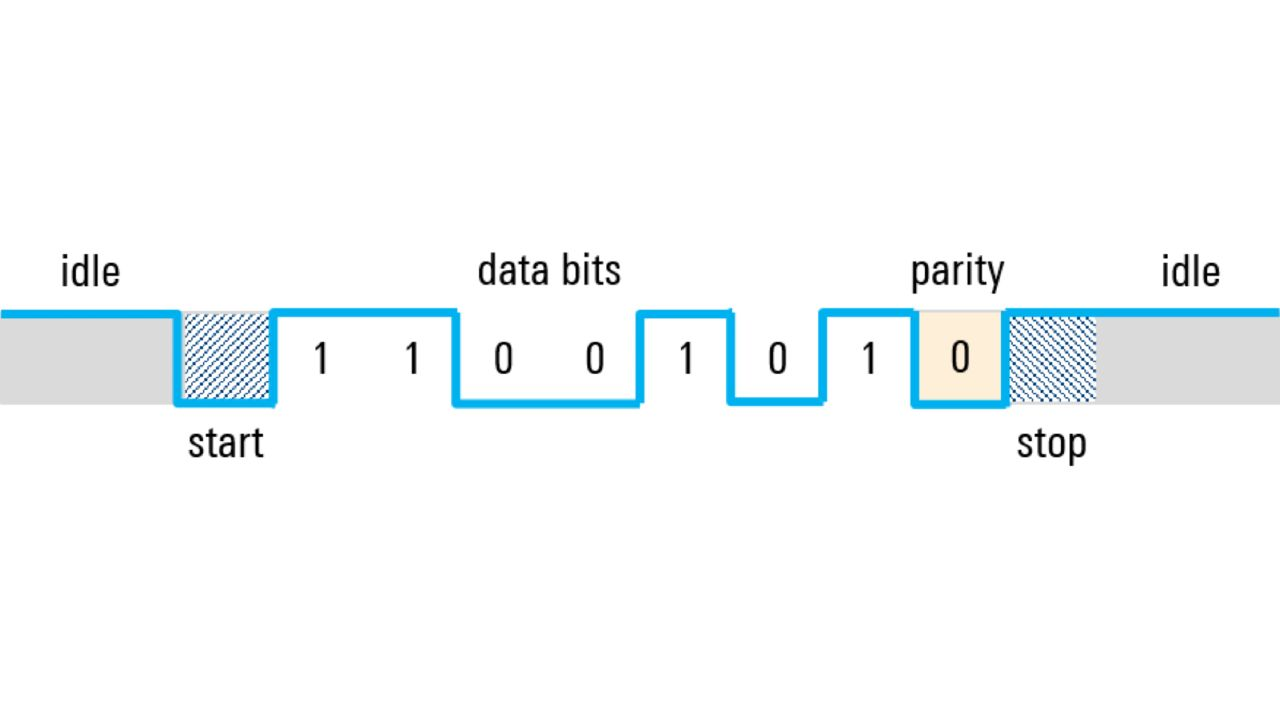
\includegraphics[width=0.8\textwidth]{Pictures/UART-Frame.jpg}
    \caption{Rahmenformat von UART. Quelle: \url{https://cdn.rohde-schwarz.com/image/products/test-and-measurement/essentials-test-equipment/essentials-digital-oscilloscopes/understanding-uart-02-infographic-rohde-schwarz_200_112521_1024_576_7.jpg}}
    \label{fig:UART-Frame}
\end{figure}
\clearpage
Die Übertragung erfolgt in Form von Bytes, die aus 8 Datenbits bestehen. UART-Rahmen enthalten Start- und Stoppbits und Datenbits, die die tatsächliche Information tragen. Wie bei den meisten digitalen Systemen ist es vom UART-Protokoll festgelegt, dass der HIGH-Pegel einer logischen $"1"$ und der LOW-Pegel einer logischen $"0"$ entspricht. Eine spezifische Spannungsschwelle ist aus Flexibilitätsgründen durch UART nicht festgelegt, weswegen der HIGH-Pegel als $"Mark"$ und der LOW-Pegel als $"$Space$"$ beschrieben wird. Doch es ist zu beachten, dass das System beim UART-Protokoll im Ruhezustand (engl. idle) bei einem HIGH-Pegel liegt. Dies hat den Sinn, dass man bei einer beschädigten Leitung durch einen konstanten LOW-Pegel im Ruhezustand eine defekte Leitung/Verbindung bzw. einen defekten Sender erkennen kann.\footnote{Vgl. Rohde \& Schwarz: UART verstehen. Online: \url{https://www.rohde-schwarz.com/de/produkte/messtechnik/essentials-test-equipment/digital-oscilloscopes/uart-verstehen_254524.html} (abgerufen am 07.07.2025).}

Der Startbit signalisiert den Beginn der Datenübertragung. Hierbei übergeht der Sender aus dem Ruhezustand (HIGH-Pegel) in den LOW-Pegel, um dem Empfänger zu signalisieren, dass die Datenübertragung beginnt. 
Unmittelbar danach folgen die Datenbits, die das Nutzsignal übertragen. Die Datenbits werden nacheinander gesendet, wobei eine Übertragung von 5 bis 9 Bits pro Byte erlaubt ist, jedoch eine Übertragung von 7 oder 8 Bits pro Byte am häufigsten verwendet wird. Die Reihenfolge der Datenbits wird dabei vom Sender invertiert und mit dem Least Significant Bit (LSB) zuerst gesendet. Das Most Significant Bit (MSB) wird zuletzt gesendet.
Nach einer erfolgreichen Übertragung der Nutzdaten übergeht der Sender zurück in den Ruhezustand (HIGH-Pegel), um dem Empfänger zu signalisieren, dass die Übertragung abgeschlossen ist.
In einigen Fällen kann es auch vorkommen, dass ein zweites (optionales) Stoppbit konfiguriert wird, um dem Empfänger Zeit für den nächsten Übertragungsrahmen zu gewähren. Dies wird jedoch in der Praxis selten umgesetzt.\footnote{Vgl. Rohde \& Schwarz: UART verstehen. Online: \url{https://www.rohde-schwarz.com/de/produkte/messtechnik/essentials-test-equipment/digital-oscilloscopes/uart-verstehen_254524.html} (abgerufen am 07.07.2025).}

Zuletzt sollte man noch erwähnen, dass manchmal ein Paritätsbit zur Verwendung kommt. Dieses trägt zur Fehlererkennung bei, indem es die Anzahl der gesetzten Bits (1-Bits) in einem Byte überprüft. Es gibt zwei Arten von Paritätsbits: 
\begin{itemize}
    \item Gerade Parität: Hier wird das Paritätsbit so gesetzt, dass die Gesamtanzahl der 1-Bits im Byte gerade ist.
    \item Ungerade Parität: Hier wird das Paritätsbit so gesetzt, dass die Gesamtanzahl der 1-Bits im Byte ungerade ist.
\end{itemize}

Das Paritätsbit kann jedoch nur ein einziges gekipptes (also falsch übertragenes) Bit erkennen, aber nicht korrigieren. Es kann auch nicht erkennen, ob zwei oder mehr Bits gekippt wurden. Daher ist es in der Praxis nicht sehr verbreitet und wird oft weggelassen.\footnote{Vgl. ebenda}

Bei unserer tatsächlichen Schaltung liegt auch ein Standard-UART-Protokoll vor, das eine Baudrate von 115200 Baud und eine Datenübertragung von 8 Datenbits verwendet.

\subsubsection{Betriebsarten von UART}
Es gibt insgesamt drei Arten des Betriebs des UART-Protokolls:
\begin{enumerate}
    \item \textbf{Simplex-Betrieb}: Die Daten werden nur in eine Richtung gesendet.
    \item \textbf{Halbduplex-Betrieb}: Jede Seite sendet, aber nicht zur selben Zeit.
    \item \textbf{Vollduplex-Betrieb}: Beide Seiten können gleichzeitig senden.
\end{enumerate}

Im vorliegenden Versuchsaufbau liegt ein Simplex-Betrieb vor. 
Trotzdem muss man erwähnen, dass der Sender aufgrund der Jumperkonfiguration auch die Daten selbst empfangen kann.

\section{BER}
Bit Error Rate (BER) oder auf Deutsch Bitfehlerrate ist eine Angabe, die die
Anzahl der falsch empfangenen Bits ins Verhältnis zu den insgesamt empfangenen Bits setzt.
\begin{equation}
    BER = \frac{N_{\text{Anzahl fehlerhaft empfangener Bits}}}{N_{\text{Anzahl empfangener Bits}}}
\end{equation}
\subsection{Beispiel}
Wir betrachten ein Beispiel: Folgende Sequenz wird gesendet:
\begin{equation}
    10111001
\end{equation}
Empfangen wurde aber:
\begin{equation}
      10\textcolor{red}{0}1\textcolor{red}{0}0\textcolor{red}{1}1
\end{equation}
Es ist schnell zu erkennen, dass hier drei Bits falsch empfangen wurden.
Die Bitfehlerrate beträgt in diesem Fall:
\begin{equation}
    BER = \frac{3}{8} = 0{,}375
\end{equation}
\subsubsection{Matlab}
\begin{figure}[H]
    \centering
    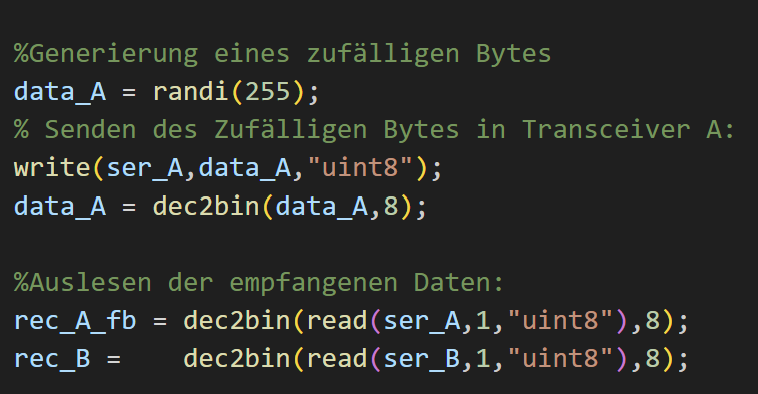
\includegraphics[width=0.5\textwidth]{Pictures/einlesenMatlab.png}
    \caption{Senden/Empfangen}
    \label{fig:matlab_example}
\end{figure}
In diesem Code wird zuerst eine Zufallszahl erzeugt, die bis 255 geht.
Um diese in binärer Form darzustellen, werden 8 Bit benötigt.
\\
Nachdem die Daten gesendet wurden, werden sie vom Empfänger und auch Sender eingelesen.
Danach werden sie in die Variable rec\_A\_fb für den Sender selbst und rec\_B für den Empfänger gespeichert.
\\
Nun wird genauer betrachtet, wie die Bitfehlerrate berechnet wird:
\begin{figure}[H]
    \centering
    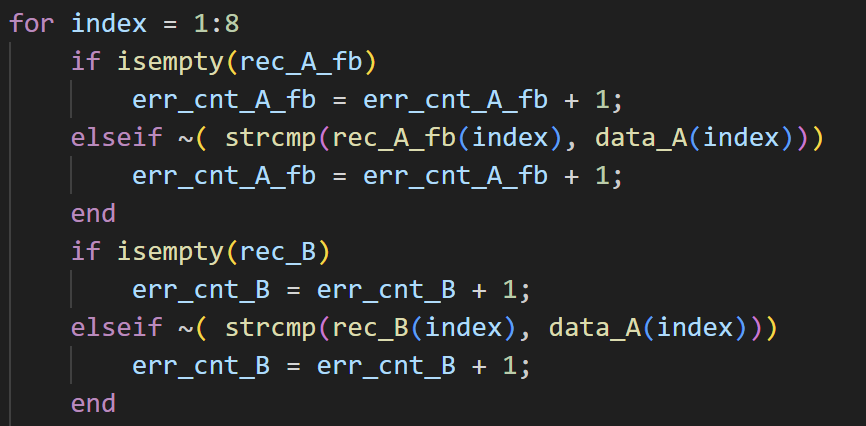
\includegraphics[width=0.5\textwidth]{Pictures/vergleich.png}
    \caption{Bitfehlerrate-Berechnung}
    \label{fig:bitfehler}
\end{figure}
Wir iterieren über jedes Bit, also insgesamt acht Mal.
Die Fehleranzahl wird in err\_cnt\_A\_fb und err\_cnt\_B gespeichert.
Konnten gar keine Daten empfangen werden, wird der jeweilige Counter auf 8 hochgezählt.
Der zentrale Part ist das bitweise Vergleichen der gesendeten und empfangenen Daten.
Stimmen diese nicht überein, wird ebenfalls der Error-Counter hochgezählt.
Zum Schluss wird die BER berechnet und ausgegeben.
Um die Genauigkeit zu erhöhen, wird das mehrfach wiederholt, ebenso wird auch der Sender und Empfänger vertauscht.
Das wurde hier der Übersichtlichkeit und Symmetrie halber nicht genauer betrachtet.

\section{Pegelplanrechnung}
Das Ziel der Pegelplanrechnung ist, den Abstand zu berechnen, der noch reicht, um die Daten zu empfangen.
Das heißt, am Ende der Empfängerkette muss ein stark genuges Signal ankommen, dass der Komparator schalten kann.
Dafür wird die Schaltung von hinten nach vorne analysiert, um herauszufinden, welche Leistung am Empfänger anliegen muss, damit der Komparator schaltet.

Aus Versuch fünf ist die Komparator-Schwellspannung, die bei etwa $U_{\text{Schwell}} = 0{,}822~\mathrm{V}$ liegt, bekannt.

Als Nächstes können wir mithilfe der Analogverstärker-Kennlinie bzw. der Übertragungsfunktion die Spannung am Kondensator C22 berechnen.
Wenn wir ein Ausgangssignal von $U_{\text{out}} = 0{,}822~\mathrm{V}$ annehmen, können wir die Eingangsspannung $U_{\text{in}}$ berechnen.
Die Übertragungsfunktion $\frac{U_{\text{out}}}{U_{\text{in}}}=\frac{U_{\text{out}}}{U_{C22}}$ lautet wie folgt (im linearen Bereich):
\begin{equation}
    U_{\text{out}} = 7{,}36 \cdot U_{C22} -1{,}63~\mathrm{V}
\end{equation}
Aufgelöst nach $U_{C22}$ ergibt sich:
\begin{equation}
    U_{C22} = \frac{U_{\text{out}} + 1{,}63~\mathrm{V}}{7{,}36} = \frac{0{,}822~\mathrm{V} + 1{,}63~\mathrm{V}}{7{,}36} = 0{,}333~\mathrm{V}
\end{equation}

Die Formel der Sensitivität aus Versuch fünf:
\begin{equation}
    U_{\text{C22}} = k \cdot \sqrt{P_{\text{in}}} - U_{\text{offset}}
\end{equation}
Umgestellt nach $P_{\text{in}}$ ergibt sich:
\begin{equation}
    P_{\text{in}} = \left(\frac{U_{\text{C22}} + U_{\text{offset}}}{k}\right)^2
\end{equation}
Mit den empirisch bestimmten Werten und dem vorher berechneten Wert für $U_{C22}$ ergibt sich:
\begin{equation}
    P_{\text{min}} = 10 \cdot \log\left(\left(\frac{0{,}333~\mathrm{V} + 0{,}36827~\mathrm{V}}{9{,}72~\frac{\mathrm{V}}{\sqrt{\mathrm{mW}}}}\right)^2\right) = -22{,}84~\mathrm{dBm}
\end{equation}
Somit wissen wir nun, welche Leistung am Eingang des Empfängers anliegen muss, damit ein gesendetes Signal auch empfangen werden kann.
Jetzt berechnen wir den Path-Loss, den wir maximal haben dürfen, um danach die maximale Reichweite zu ermitteln.
Die maximale Freiraumdämpfung (Path-Loss) wird mit folgender Formel berechnet:
\begin{equation}
    D_{\text{Path}} = P_{\text{TXGemessen}} + D_{\text{Kabel}} + G_{\text{TXAntenna}} + G_{\text{RXAntenna}} - P_{\text{RXMin}}
\end{equation}
\begin{equation}
    D_{\text{Path}} = -7{,}7~\mathrm{dBm} + 0{,}45~\mathrm{dB} -0{,}51~\mathrm{dBi} -0{,}51~\mathrm{dBi} - (-22{,}84~\mathrm{dBm}) = 14{,}57~\mathrm{dB}
\end{equation}
\begin{equation}
    D_{\text{Path}} = 20 \cdot \log\left(\frac{4 \pi d f}{c}\right)
\end{equation}
Umgestellt nach $d$ ergibt sich:
\begin{equation}
    d = \frac{c}{4 \pi f} \cdot 10^{\frac{D_{\text{Path}}}{20}}=0{,}102~\mathrm{m} 
\end{equation}
Somit erhalten wir eine maximale Reichweite von $d = 0{,}102~\mathrm{m}$. Der Abstand müsste etwas kleiner sein, damit der Komparator schaltet,
sonst liegt man exakt auf der Schwellspannung.
In der Realität hatten wir eine maximale gesicherte Funkreichweite von $d_{\text{TR,max}}=8~\mathrm{cm}$.
Teilweise konnte sogar eine Reichweite von $9~\mathrm{cm}$ erzielt werden.
Die kleine Abweichung zum berechneten Wert ist auf verschiedene Faktoren zurückzuführen, wie z.\,B. die Ungenauigkeit der approximierten Funktionen, Messungenauigkeiten und zusätzliche Übertragungsfehler.
In der Realität hatten wir eine maximale gesicherte Funkreichweite von $d_{TR,max}=8cm$.
Teilweise konnte sogar eine Reichweite von $9cm$ erzielt werden.
Die kleine Abweichung zum berechneten Wert ist auf verschiedene Faktoren zurückzuführen, wie z.B. die Ungenauigkeit der approximierten Funktionen, Messungenauigkeiten und zusätzliche Übertragungsfehler.

